\documentclass{article}
\usepackage[paperwidth=24cm,paperheight=12cm,margin=0.3cm]{geometry}
\usepackage{amsmath}
\usepackage{tikz}
\usetikzlibrary{arrows.meta,positioning,fit,backgrounds}
\pagestyle{empty}

\begin{document}
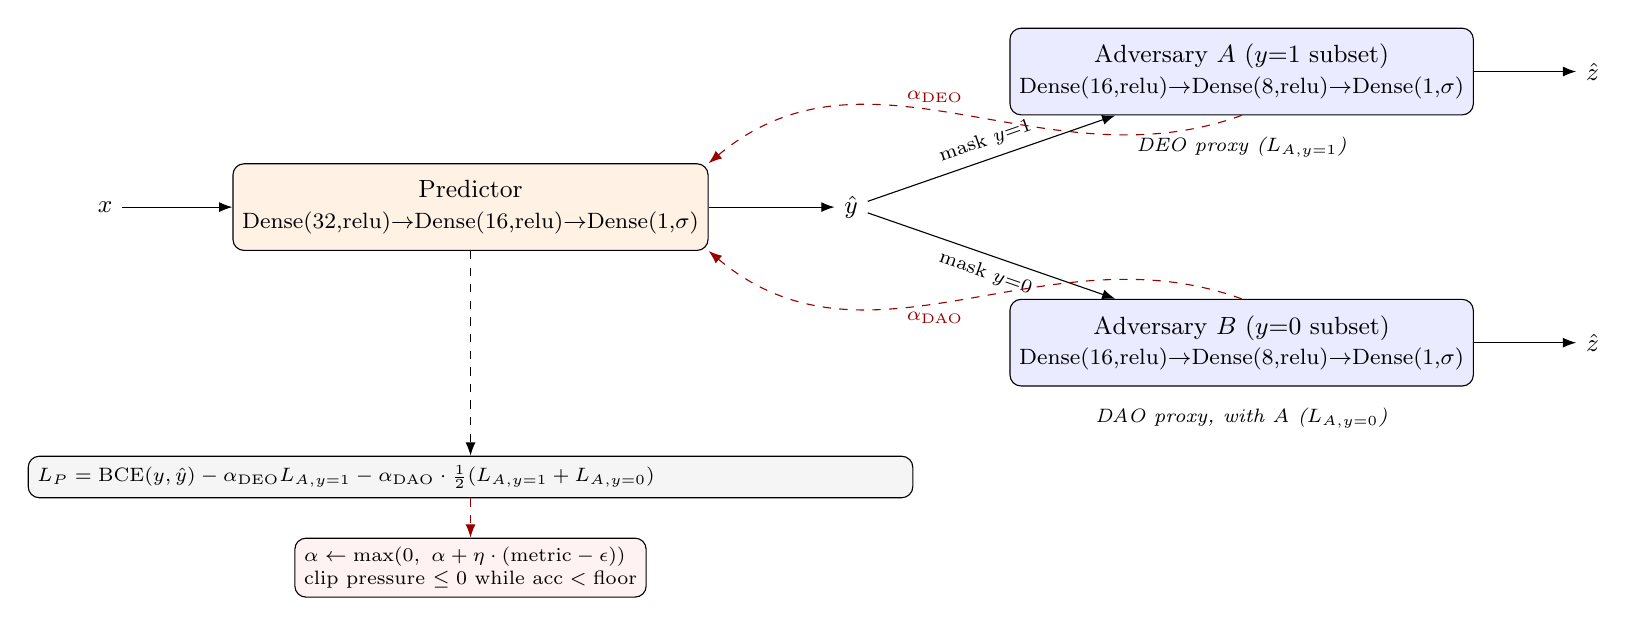
\begin{tikzpicture}[
  font=\small,
  box/.style={draw, rounded corners, align=center, minimum height=1.1cm, minimum width=2.6cm, fill=blue!5},
  predbox/.style={box, fill=orange!10, minimum width=3.2cm},
  advbox/.style={box, fill=blue!8},
  sig/.style={draw, circle, minimum size=0.6cm, fill=white},
  -{Latex[length=2.2mm]},
  >=Latex,
  node distance=1.0cm and 1.4cm
]

% --- predictor ---
\node[predbox] (pred) {Predictor\\ \footnotesize Dense(32,relu)$\to$Dense(16,relu)$\to$Dense(1,$\sigma$)};

\node[left=1.4cm of pred] (x) {$x$};
\draw[-{Latex}] (x) -- (pred);

\node[right=1.6cm of pred] (yhat) {$\hat{y}$};
\draw[-{Latex}] (pred) -- (yhat);

% --- split into masked subsets ---
\node[advbox, above right=0.9cm and 1.8cm of yhat] (adv1) {Adversary $A$ ($y{=}1$ subset)\\ \footnotesize Dense(16,relu)$\to$Dense(8,relu)$\to$Dense(1,$\sigma$)};
\node[advbox, below right=0.9cm and 1.8cm of yhat] (adv0) {Adversary $B$ ($y{=}0$ subset)\\ \footnotesize Dense(16,relu)$\to$Dense(8,relu)$\to$Dense(1,$\sigma$)};

\draw[-{Latex}] (yhat) -- node[above,sloped,font=\scriptsize]{mask $y{=}1$} (adv1);
\draw[-{Latex}] (yhat) -- node[below,sloped,font=\scriptsize]{mask $y{=}0$} (adv0);

\node[right=1.3cm of adv1] (zhat1) {$\hat{z}$};
\node[right=1.3cm of adv0] (zhat0) {$\hat{z}$};
\draw[-{Latex}] (adv1) -- (zhat1);
\draw[-{Latex}] (adv0) -- (zhat0);

\node[below=0.15cm of adv1, font=\scriptsize\itshape] {DEO proxy ($L_{A,y=1}$)};
\node[below=0.15cm of adv0, font=\scriptsize\itshape] {DAO proxy, with $A$ ($L_{A,y=0}$)};

% --- feedback: dual ascent ---
\draw[dashed, -{Latex}, red!60!black] (adv1.south) to[out=200,in=40] node[above,font=\scriptsize,pos=0.55]{$\alpha_{\text{DEO}}$} (pred.north east);
\draw[dashed, -{Latex}, red!60!black] (adv0.north) to[out=160,in=-40] node[below,font=\scriptsize,pos=0.55]{$\alpha_{\text{DAO}}$} (pred.south east);

% --- loss box ---
\node[draw, rounded corners, fill=gray!8, below=2.6cm of pred, align=left, font=\scriptsize, text width=11cm] (loss) {
  $L_P = \text{BCE}(y,\hat{y}) - \alpha_{\text{DEO}} L_{A,y=1} - \alpha_{\text{DAO}} \cdot \tfrac{1}{2}(L_{A,y=1}+L_{A,y=0})$
};
\draw[dashed,-{Latex}] (pred.south) -- (loss.north);

% --- dual ascent update box ---
\node[draw, rounded corners, fill=red!5, below=0.5cm of loss, align=left, font=\scriptsize] (update) {
  $\alpha \leftarrow \max(0,\ \alpha + \eta\cdot(\text{metric} - \epsilon))$ \\
  clip pressure $\leq 0$ while $\text{acc} < \text{floor}$
};
\draw[dashed,-{Latex}, red!60!black] (loss.south) -- (update.north);

\end{tikzpicture}
\end{document}
